\section*{Đề kiểm tra Chương 7}
\subsection*{Đề số 1}
\setcounter{ex}{0}\setcounter{bt}{0}
\Opensolutionfile{ans}[ans/ans-KT-701]
\noindent\textbf{I. PHẦN TRẮC NGHIỆM}
\begin{ex}%[0H3Y2-1]%[Yến Trần BG10]
	Đường tròn $x^2 + y^2 + 4x- 8y - 5 = 0$ có tọa độ tâm $I$ và bán kính $R$ là
	\choice
	{$I(-2;4)$, $R = \sqrt{5}$}
	{\True $I(-2;4)$, $R = 5$}
	{$I(2;-4)$, $R = \sqrt{5}$}
	{$I(2;-4)$, $R = 5$}
	\loigiai
	{
		Đường tròn $x^2 + y^2 + 4x- 8y - 5 = 0$ có tọa độ tâm $I(-2;4)$, bán kính $R = 5$.
	}
\end{ex}

\begin{ex}%[0H3Y1-2]%[Yến Trần BG10]
	Đường thẳng đi qua điểm $A(1; 2)$, nhận $\vec{n}=(2;-4)$ làm véc-tơ pháp tuyến có phương trình là
	\choice
	{$x-2y-4=0$}
	{$x+y+4=0$}
	{$-x+2y-4=0$}
	{\True $x-2y+3=0$}
	\loigiai{ 
		Do đường thẳng đi qua điểm $A(1; 2)$ và nhận $\vec{n}=(2;-4)$ làm véc-tơ pháp tuyến  nên có phương trình là
		$$2(x-1)-4(y-2)=0 \Leftrightarrow 2x-4y+6=0 \Leftrightarrow x-2y+3=0.$$
	}
\end{ex}	
	
	\begin{ex}%[0H3K1-6]%[Yến Trần BG10]
		Cho đường thẳng $\Delta\colon\heva{&x=3-2t \\ &y=-1+t}$ và đường thẳng $d\colon 3x-4y-8=0$. Điểm $M(a;b)$ thuộc $\Delta$ sao cho khoảng cách từ $A$ đến $d$ bằng $3$. Biết $a$ dương, tính $T=a-b$.
		\choice
		{$T=1$}
		{$T=9$}
		{$T=2$}
		{\True $T=7$}
		\loigiai{
			Vì $M$ thuộc $\Delta$ và có $a>0$ nên $M(3-2t;-1+t)$ với điều kiện $3-2t>0\Rightarrow t<\dfrac{3}{2}$.\\
			Theo đề ta có
			\begin{eqnarray*}
				\mathrm{d}(M,d)=3&\Leftrightarrow&\dfrac{\left|3(3-2t) -4(-1+t)-8\right| }{\sqrt{3^2+(-4)^2}}=3\\
				&\Leftrightarrow&\dfrac{\left| 5-10t\right| }{5}=3\\
				&\Leftrightarrow&\left|5-10t \right| =15\\
				&\Leftrightarrow&\hoac{&5-10t=15\\&5-10t=-15}\\
				&\Leftrightarrow&\hoac{&t=-1\text{ (nhận)}\\&t=2\text { (loại).}}
			\end{eqnarray*}
			Với $t=-1$ suy ra $M(5;-2)$ nên $a=5$, $b=-2$.\\
			Vậy $T=a-b=5-(-2)=7$.
		}
	\end{ex}	
	
	
	\begin{ex}%[0H3B1-2]%[Yến Trần BG10]
		Trong mặt phẳng tọa độ $Oxy$, cho hai điểm $A(2;0)$, $B(0;4)$. Phương trình tổng quát của đường thẳng $AB$ là
		\choice
		{$2x+y-14=0$}
		{$2x+y-3=0$}
		{$2x+y-5=0$}
		{\True $2x+y-4=0$}
		\loigiai{
			PTĐT đi qua hai điểm $A(2;0)$, $B(0;4)$ là $\dfrac{x}{2}+\dfrac{y}{4}=1\Leftrightarrow 2x+y=4\Leftrightarrow 2x+y-4=0$.
		}
	\end{ex}

	\begin{ex}%[0H3Y1-2]%[Yến Trần BG10]
		Trong mặt phẳng tọa độ $Oxy$, đường thẳng $d$ đi qua điểm $(1; -2)$ và có vectơ chỉ phương $\overrightarrow{u}=(3; 5)$ có PTTS là 
		\choice
		{$d\colon\heva{&x=3+2t\\&y=5+t}$}
		{$d\colon\heva{&x=3+t\\&y=5-2t}$}
		{\True $d\colon \heva{&x=1+3t\\&y=-2+5t}$}
		{$d\colon \heva{&x=1+5t\\&y=-2-3t}$}
		\loigiai{
			Đường thẳng $d$ đi qua điểm $(1; -2)$ và có vectơ chỉ phương $\overrightarrow{u}=(3; 5)$ có PTTS là $d\colon \heva{&x=1+3t\\&y=-2+5t.}$
		}
	\end{ex}	
	
	\begin{ex}%[0H3B2-2]%[Yến Trần BG10]
		Viết phương trình đường tròn tâm $I\left( 3;-2 \right)$ và tiếp xúc với đường thẳng $\Delta \colon 2x-y+1=0$. 
		\choice
		{$\left( x-3 \right)^{2}+\left( y+2 \right)^{2}=\dfrac{9}{\sqrt{5}}$}
		{$\left( x-3 \right)^{2}+\left( y+2 \right)^{2}=\dfrac{9}{5}$}
		{$\left( x-3 \right)^{2}+\left( y+2 \right)^{2}=\dfrac{3}{\sqrt{5}}$}
		{\True $\left( x-3 \right)^{2}+\left( y+2 \right)^{2}=\dfrac{81}{5}$}
		\loigiai{
			Bán kính $R=\mathrm{d} \left(I,\Delta \right)=\dfrac{\left| 2.3+2+1 \right|}{\sqrt{2^2+(-1)^{2}}}=\dfrac{9}{\sqrt{5}}$. \\ 
			Đường tròn $(C)$ có tâm $I\left( 3;-2 \right)$, bán kính $R=\dfrac{9}{\sqrt{5}}$ có phương trình là $(C) \colon \left( x-3 \right)^{2}+\left( y+2 \right)^{2}=\dfrac{81}{5}$. 
		}
	\end{ex}

	\begin{ex}%[0H3B2-1]%[Yến Trần BG10]
		Xác định tâm $I$ và tính bán kính $R$ của đường tròn có phương trình $x^2+y^2+4x=0$. 
		\choice
		{$I\left( 2;0 \right)$, $R=2$}
		{\True $I\left( -2;0 \right)$, $R=2$}
		{$I\left( 2;0 \right)$, $R=\sqrt{2}$}
		{$I\left( -2;0 \right)$, $R=\sqrt{2}$}
		\loigiai{
			Phương trình tổng quát của đường tròn có dạng $x^2+y^2-2ax-2by+c=0$ với $I\left( a; b \right)$ là tâm và bán kính được tính bằng công thức $R=\sqrt{a^2+b^2-c}$. \\ 
			Ta có tọa độ tâm $I \heva{& a=\dfrac{4}{-2}=-2  \\ & b=\dfrac{0}{-2}=0}$ và bán kính $R=\sqrt{\left( -2 \right)^{2}}=2$. \\ 
		}
	\end{ex}
	

	\begin{ex}%[0H3B1-2]%[Yến Trần BG10]
		Viết PTĐT đi qua $M\left( 3;4 \right)$ và có hệ số góc $k=2$. 
		\choice
		{$y=2x-10$}
		{\True $y=2x-2$}
		{$y=2x+2$}
		{$y=2x+10$}
		\loigiai{
			PTĐT đi qua $M\left( x_0;y_0 \right)$ và có hệ số góc $k$ có dạng $y=k\left( x-x_0 \right)+y_0$. \\ 
			Do đó PTĐT đi qua $M\left( 3;4 \right)$ và có hệ số góc $k=2$ là 
			\[ y=2\left( x-3 \right)+4 \Leftrightarrow y=2x-2.\] 
		}
	\end{ex}
	
	

\begin{ex}%[0H3Y1-1]%[Yến Trần BG10]
	Cho đường thẳng có PTTS $\heva{&x=2+3t\\&y=-3-t}$ có tọa độ véc-tơ chỉ phương là
	\choice
	{$\left(2;-3\right)$}
	{\True $\left(3;-1\right)$}
	{$\left(3;1\right)$}
	{$\left(3;-3\right)$}
	\loigiai{
		Ta có PTTS của đường thẳng đi qua điểm $M\left(x_0;y_0\right)$ và có véc-tơ chỉ phương $\vec{u}=(a;b)$\\ có dạng $\heva{&x=x_0+at\\&y=y_0+bt.}$	\\
		Suy ra, véc-tơ chỉ phương $\vec{u}=(3;-1)$.
	}
\end{ex}
\begin{ex}%[0H3Y1-5]%[Yến Trần BG10]
	Khoảng cách từ điểm $M(-2;3)$ đến đường thẳng $\Delta \colon 4x+3y+4=0$ là
	\choice
	{$\dfrac{10}{\sqrt{5}}$}
	{\True $1$}
	{$\dfrac{21}{5}$}
	{$\dfrac{21}{25}$}
	\loigiai{
		Ta có $\mathrm{d}(M,\Delta) = \dfrac{|4\cdot (-2) + 3\cdot 3 + 4|}{\sqrt{4^2+3^2}} = 1$.
	}
\end{ex}
\begin{ex}%[0H3Y1-1]%[Yến Trần BG10]
	Cho đường thẳng $d \colon 4x-y+2=0$. Véc-tơ pháp tuyến của đường thẳng $d$ là
	\choice
	{$\overrightarrow{n}=(4;2)$}
	{\True $\overrightarrow{n}=(4;-1)$}
	{$\overrightarrow{n}=(1;4)$}
	{$\overrightarrow{n}=(1;-4)$}
	\loigiai{
		Ta có $\overrightarrow{n}=(4;-1)$ là một véc-tơ pháp tuyến của đường thẳng $d$.}
\end{ex}
\begin{ex}%[0H3B1-3]%[Yến Trần BG10]
	Xác định vị trí tương đối của hai đường thẳng sau đây $\Delta_1 \colon 3x-2y+4=0$ và \break $\Delta_2 \colon -6x+4y-8=0$.
	\choice
	{\True Trùng nhau}
	{Cắt nhau}
	{Song song}
	{Vuông góc nhau}
	\loigiai{
		Ta có $\dfrac{3}{-6} = \dfrac{-2}{4} = \dfrac{4}{-8} = -\dfrac{1}{2}$ nên $\Delta_1$ trùng $\Delta_2$.}
\end{ex}
\begin{ex}%[0H3B2-3]%[Yến Trần BG10]
	Phương trình tiếp tuyến tại điểm $M(2;3)$ với đường tròn $(C) \colon x^2+y^2-2x-4y+3=0$ là
	\choice
	{$x+y-3=0$}
	{\True $x+y-5=0$}
	{$x-y-5=0$}
	{$x+y+5=0$}
	\loigiai{
		Đường tròn $(C)$ có tâm $I(1;2)$ và bán kính $R = \sqrt{2}$.\\
		Gọi $\Delta$ là tiếp tuyến với $(C)$ tại $M(2;3)$.\\
		Đường thẳng $\Delta$ qua $M(2;3)$ và nhận $\vec{IM} = (1;1)$ làm véc-tơ pháp tuyến. \\
		Vậy phương trình $\Delta$ là $1(x-2) + 1(y-3) = 0 \Leftrightarrow x + y - 5 = 0$.}
\end{ex}

\begin{ex}%[0H3K1-2]%[Yến Trần BG10]
	Viết PTTS của đường thẳng $d$ qua điểm $A(4;1)$ và vuông góc với đường thẳng $\Delta \colon x-3y+4=0$.
	\choice
	{$\heva{&x=t\\&y=4+3t}$}
	{\True $\heva{&x=4+t\\&y=1-3t}$}
	{$\heva{&x=4+3t\\&y=1+t}$}
	{$\heva{&x=1+4t\\&y=2-t}$}
	\loigiai{
		Đường thẳng $\Delta \colon x-3y+4=0$ có một véc-tơ pháp tuyến $\vec{n} = (1;-3)$. \\
		Đường thẳng $d$ qua điểm $A(4;1)$ và vuông góc với $\Delta$ nên nhận $\vec{n} = (1;-3)$ làm véc-tơ chỉ phương.
		Vậy, PTTS $d \colon \heva{&x=4+t\\&y=1-3t.}$}
\end{ex}
\begin{ex}%[0H3B1-2]%[Yến Trần BG10]
	Trong mặt phẳng tọa độ $Oxy$, phương trình tổng quát của đường thẳng đi qua điểm $A(0;1)$ và có véc-tơ chỉ phương $\vec{u}=(2;5)$ là
	\choice
	{\True $5x-2y+2=0$}
	{$2x-5y-7=0$}
	{$5x-2y-7=0$}
	{$3x+2y-4=0$}
	\loigiai{
		Đường thẳng $d$ qua $A(0;1)$ và có véc-tơ chỉ phương $\vec{u}=(2;5)$ nên $d$ có một véc-tơ pháp tuyến $\vec{n} = (5;-2)$.\\
		PTĐT $d \colon 5(x-0) - 2(y-1) = 0 \Leftrightarrow 5x - 2y + 2 = 0$.	
	}
\end{ex}

\begin{ex}%[0H3Y1-1]%[Yến Trần BG10]
	Tìm một véc-tơ chỉ phương của đường thẳng $d \colon \heva{&x=2+3t\\&y=4.}$
	\choice
	{$\overrightarrow{u}_4=(0;1)$}
	{$\overrightarrow{u}_2=(3;4)$}
	{$\overrightarrow{u}_3=(2;4)$}
	{\True $\overrightarrow{u}_1=(1;0)$}
	\loigiai{
		Đường thẳng $d \colon \heva{&x=2+3t\\&y=4}$ có một véc-tơ chỉ phương là $\vec{v} = (3;0)$.\\
		Ta có $\vec{v} = 3 \vec{u}_1$ nên $\vec{u}_1$ cũng là véc-tơ chỉ phương của $d$.	
	}
\end{ex}
\begin{ex}%[0H3K1-2]%[Yến Trần BG10]
	Cho $A(1;2)$ và $\Delta \colon 2x+y+1=0$. Đường thẳng $d$ đi qua điểm $A$ và song song với $\Delta$ có phương trình là
	\choice
	{$2x+y+5=0$}
	{$x-2y-5=0$}
	{\True $2x+y-4=0$}
	{$2x+y=0$}
	\loigiai{
		Đường thẳng $d$ qua $A(1;2)$ và song song với $\Delta \colon 2x+y+1=0$ nên có phương trình 
		\[2(x-1) + (y-2) = 0 \Leftrightarrow 2x + y - 4 = 0. \]}
\end{ex}
\begin{ex}%[0H3Y1-4]%[Yến Trần BG10]
	Tính góc giữa hai đường thẳng $d \colon 2x-5y+2=0$ và $\Delta \colon 5x+2y-4=0$.
	\choice
	{\True $90^\circ$}
	{$60^\circ$}
	{$30^\circ$}
	{$45^\circ$}
	\loigiai{
		Đường thẳng $d$ có véc-tơ pháp tuyến $\vec{u} = (2;-5)$, đường thẳng $\Delta$ có véc-tơ chỉ phương $\vec{v} = (5;2)$.\\
		Ta có $\vec{u} \cdot \vec{v} = 2\cdot 5 + (-5)\cdot 2 = 0$ nên $d\perp \Delta$.}
\end{ex}


\begin{ex}%[0H3B2-2]%[Yến Trần BG10]
	Đường tròn $(C)$ đi qua hai điểm $A(1;1)$, $B(3;5)$, và có tâm $I$ thuộc trục tung có phương trình là
	\choice
	{$x^2+y^2+4y+6=0$}
	{$x^2+(y-4)^2=6$}
	{$x^2+(y+4)^2=6$}
	{\True $x^2+y^2-8y+6=0$}
	\loigiai{
		$I \in Oy \Rightarrow I(0;y)$. $\vec{IA} = (1;1-y)$, $\vec{IB} = (3; 5-y)$.\\
		Ta có $IA = IB \Leftrightarrow IA^2 = IB^2 \Leftrightarrow 1^2 + (1-y)^2 = 3^2 + (5-y)^2 \Leftrightarrow y = 4$. \\
		Suy ra $I(0;4)$, $R = IA = \sqrt{1^2 + (1-4)^2} = \sqrt{10}$. \\
		Phương trình đường tròn $(C)\colon x^2 + (y-4)^2 = 10 \Leftrightarrow x^2 + y^2 - 8y + 6 = 0$.	
	}
\end{ex}
\begin{ex}%[0H2Y2-3]%[Yến Trần BG10]
	Hai véc-tơ chỉ phương và véc-tơ pháp tuyến của một đường thẳng
	\choice
	{Song song với nhau}
	{\True Vuông góc với nhau}
	{Trùng nhau}
	{Bằng nhau}
	\loigiai{Ta có hai véc-tơ chỉ phương và véc-tơ pháp tuyến của một đường thẳng vuông góc với nhau.}
\end{ex}

	\begin{ex}%[0H3B2-2]%[Yến Trần BG10]
	Trong mặt phẳng tọa độ $ Oxy $, cho tam giác $ ABC $ với $ A(1;0) $, $ B(1;-4) $ và $ C(3;-2) $. Đường tròn ngoại tiếp tam giác $ ABC $ có phương trình là
	\choice
	{\True $ x^2+y^2-2x+4y+1=0 $}
	{$ x^2+y^2-20x-14y+19=0 $}
	{$ x^2+y^2+5x+4y-6=0 $}
	{$ x^2+y^2-x+3y-4=0 $}
	\loigiai
	{Gọi phương trình đường tròn ngoại tiếp tam giác $ ABC $ là $ x^2+y^2-2ax-2by+c=0 $ với $ a , b ,c\in \mathbb{R} $.\\
		Do đường tròn đi qua 3 điểm $ A , B $ và $ C $ nên ta có hệ phương trình
		$$ \heva{& 1^2+0^2-2a \cdot 1 -2b \cdot 0 +c =0 \\ & 1^2+(-4)^2-2a \cdot 1 -2b \cdot (-4) +c =0 \\ & 3^2+(-2)^2-2a \cdot 3 -2b \cdot (-2) +c =0} \Leftrightarrow \heva{& -2a+c=-1 \\ & -2a+8b+c =-17 \\ & -6a+4b+c=-13} \Leftrightarrow \heva{& a=1 \\ &b=-2 \\ &c=1.}$$
		Phương trình đường tròn cần tìm là $ x^2+y^2-2x+4y+1=0 $.
	}
\end{ex}
\begin{ex}%[0H3B1-2]%[Yến Trần BG10]
	Trong mặt phẳng $Oxy$, cho $\Delta$ có PTTS $\heva{&x=1-3t \\ &y=2+t}$. Phương trình tổng quát của đường thẳng $\Delta$ là
	\choice
	{$3x-y-7=0$}
	{$x+3y+5=0$}
	{\True $x+3y-7=0$}
	{$3x+y+5=0$}
	\loigiai{
		Từ PTTS của đường thẳng $\Delta$, ta có $\Delta$ đi qua $A(1;2)$.\\
		Mặt khác, $\Delta$ nhận $\overrightarrow{u}=(-3;1)$ làm véc-tơ chỉ phương nên nhận $\overrightarrow{n}=(1;3)$ làm véc-tơ pháp tuyến.\\
		Do đó, ta có phương trình
		\[(x-1)+3(y-2)=0 \Leftrightarrow x+3y-7=0.\]
	}
\end{ex}


\begin{ex}%[0H3Y3-1]%[Yến Trần BG10]
	Trong mặt phẳng $Oxy$, phương trình nào sau đây là phương trình elip?
	\choice
	{$\dfrac{x}{9}+\dfrac{y}{4}=1$}
	{$\dfrac{x^2}{9}+\dfrac{y^2}{4}=0$}
	{\True $\dfrac{x^2}{9}+\dfrac{y^2}{4}=1$}
	{$\dfrac{x^2}{9}-\dfrac{y^2}{4}=1$}
	\loigiai{
		Phương trình elip có dạng $\dfrac{x^2}{a^2}+\dfrac{y^2}{b^2}=1$ nên ta chọn phương án đúng là $\dfrac{x^2}{9}+\dfrac{y^2}{4}=1$.
	}
\end{ex}	
	\begin{ex}%[0H3B1-2]%[Yến Trần BG10]
		Viết phương trình tổng quát của đường cao đỉnh $A$ của tam giác $ABC$ biết toạ độ các đỉnh $A\left( 3;4 \right)$, $B\left( -2;5 \right)$, $C\left( 7;7 \right)$.
		\choice
		{$9x-2y-19=0$}
		{\True $9x+2y-35=0$}
		{$2x+9y-42=0$}
		{$2x-9y+30=0$}
		\loigiai{
			Gọi $d$ là đường cao từ đỉnh $A$ của tam giác $ABC$, khi đó $d \perp BC$. \\
			Suy ra một véc-tơ pháp tuyến của $d$ là $\overrightarrow{n_{d}}=\overrightarrow{BC}=\left( 9;2 \right)$. \\ 
			Vậy phương trình tổng quát của đường thẳng $d$ đi qua $A$ và có véc-tơ pháp tuyến $\overrightarrow{n_{d}}=\left( 9;2 \right)$ là 
			\[ 9 \left( x-3 \right)+2\left( y-4 \right)=0 \Leftrightarrow 9x+2y-35=0. \]
		}
	\end{ex}

	\begin{ex}%[0H3B1-2]%[Yến Trần BG10]
	Véc-tơ nào dưới đây là một véc-tơ chỉ phương của đường thẳng song song với trục $Oy$?
		\choice
	{\True $\overrightarrow{u_{1}}=(0;1)$}
	{$\overrightarrow{u_{2}}=(0;-1)$}
	{$\overrightarrow{u_{3}}=(-1;1)$}
	{$\overrightarrow{u_{4}}=(1;1)$}
	\loigiai{
		Trục $ Ox \colon y=0$ có VTCP $\overrightarrow{i}=(0;1)$ nên một đường thẳng song song với $Ox$ cũng có  VTCP $\overrightarrow{i}=(0;1)$.
	}
\end{ex}
	\begin{ex}%[0H3B1-2]%[Yến Trần BG10]
	Véc-tơ nào dưới đây là một véc-tơ chỉ phương của đường phân giác góc phần tư thứ nhất?
		\choice
	{\True $\overrightarrow{u_{1}}=(1;1)$}
	{$\overrightarrow{u_{2}}=(0;-1)$}
	{$\overrightarrow{u_{3}}=(-1;1)$}
	{$\overrightarrow{u_{4}}=(0;1)$}
	\loigiai{
		Đường phân giác của góc phần tư thứ nhất là $x-y=0$ suy ra VTPT $\overrightarrow{n}=(1;-1)$ suy ra VTCP $\overrightarrow{u}=(1;1)$.
	}
\end{ex}

	\begin{ex}%[0H3B1-2]%[Yến Trần BG10]
	Đường thẳng $d$ đi qua điểm $M(1;-2)$ và có  véc-tơ chỉ phương là $\overrightarrow{u}=(3;5)$ có PTTS là
		\choice
	{$d \colon \heva{&x=3+t\\&y=5-2t}$}
	{\True $d \colon \heva{&x=1+3t\\&y=-2+5t}$}
	{$d \colon \heva{&x=1+5t\\&y=-2-3t}$}
	{$d \colon \heva{&x=3+2t\\&y=5+t}$}
	\loigiai{
	Ta có $M(1;-2)$ và $\overrightarrow{u_{d}}=(3;5)$ suy ra PTTS $d \colon \heva{&x=1+3t\\&y=-2+5t}$.
	}
\end{ex}

\begin{ex}%[0H3B1-2]%[Yến Trần BG10]
	Trong mặt phẳng với hệ tọa độ $Oxy$ cho ba điểm $A(3;2)$, $P(4;0)$ và $Q(0;-2)$. Đường thẳng đi qua điểm $A$ và song song với $PQ$ có PTTS là
		\choice
	{$\heva{&x=3+4t\\&y=2-2t}$}
	{$\heva{&x=3-2t\\&y=2+t}$}
	{\True $\heva{&x=-1+2t\\&y=t}$}
	{$\heva{&x=-1+2t\\&y=-2+t}$}
		\loigiai{ Gọi $d$ là đường thẳng đi qua $A$ và song song với $PQ$.\\
			Ta có $\heva{&A(3;2) \in d\\& \overrightarrow{u_{d}}=\overrightarrow{PQ}=(-4;-2)=-2(2;1)} \Rightarrow d \colon \heva{&x=3+2t\\&y=2+t}$.\\
			Với $t=-2$ suy ra $M(-1;0) \in d$.\\
			Suy ra  $d \colon \heva{&x=-1+2t\\&y=t}$.
	}
\end{ex}


\begin{ex}%[0H3B1-2]%[Yến Trần BG10]
Xét vị trí tương đối của hai đường thẳng $d_{1} \colon 3x-2y-6=0$ và $d_{2} \colon 6x-2y-8=0$.
	\choice
	{Trùng nhau}
	{Song song với nhau}
	{Vuông góc với nhau}
	{\True Cắt nhau nhưng không vuông góc}
	\loigiai{ Ta có $\heva{&d_{1} \colon 3x-2y-6=0 \Rightarrow \overrightarrow{n_{1}}=(3;-2)\\&d_{2} \colon 6x-2y-8=0 \Rightarrow \overrightarrow{n_{2}}=(6;-2)} \Rightarrow \heva{&\dfrac{3}{6} \ne \dfrac{-2}{-2}\\& \overrightarrow{n_{1}}\cdot \overrightarrow{n_{2}} \ne 0} \Rightarrow$ $d_{1}, d_{2}$ cắt nhau nhưng không vuông góc.
	}
\end{ex}
\begin{ex}%[0H3B1-2]%[Yến Trần BG10]
	Đường thẳng nào sau đây không có điểm chung với đường thẳng $x-3y+4=0$.
	\choice
{$\heva{&x=1+t\\&y=2+3t}$}
{$\heva{&x=1-t\\&y=2+3t}$}
{$\heva{&x=1-3t\\&y=2+t}$}
{\True $\heva{&x=1-3t\\&y=2-t}$}
	\loigiai{ Kí hiệu $d \colon x-3y+4=0 \Rightarrow \overrightarrow{n_{d}}=(1;-3)$.\\
		\begin{itemize}
			\item Xét đáp án A: $d_{1}\colon \heva{&x=1+t\\&y=2+3t} \Rightarrow \overrightarrow{n_{1}}=(1;3) \Rightarrow \overrightarrow{n_{1}}, \overrightarrow{n}$ không cùng phương nên loại A.
			\item Xét đáp án B: $d_{2}\colon \heva{&x=1-t\\&y=2+3t} \Rightarrow \overrightarrow{n_{2}}=(3;1) \Rightarrow \overrightarrow{n_{2}}, \overrightarrow{n}$ không cùng phương nên loại B.
		\item Xét đáp án C: $d_{3}\colon \heva{&x=1-3t\\&y=2+t} \Rightarrow \overrightarrow{n_{3}}=(1;3) \Rightarrow \overrightarrow{n_{3}}, \overrightarrow{n}$ không cùng phương nên loại B.
		\item Xét đáp án D: $d_{4}\colon \heva{&x=1-3t\\&y=2-t} \Rightarrow \heva{&\overrightarrow{n_{4}}=(3;1)\\ &M(1;2) \in d_{4}}  \Rightarrow \heva{&\overrightarrow{n_{4}}=\overrightarrow{n} \\ & M \notin d} \Rightarrow d \parallel d_{4}$.
		\end{itemize}
	}
\end{ex}

\begin{ex}%[0H3B1-2]%[Yến Trần BG10]
	Trong mặt phẳng với hệ tọa độ $Oxy$, cho hai đường thẳng có phương trình $d_{1} \colon mx+(m-1)y+2m=0$ và $d_{2} \colon 2x+y-1=0$. Nếu $d_{1}$ song song $d_{2}$ thì 
	\choice
	{\True $m=2$}
	{$m=-1$}
	{$m=-2$}
	{$m=1$}
	\loigiai{ Ta có $\heva{&d_{1} \colon mx+(m-1)y+2m=0 \\&d_{2} \colon 2x+y-1=0} \Rightarrow \heva{&m \ne 0\\& m=2m-2} \Rightarrow$ $m=2$. 
	}
\end{ex}

\begin{ex}%[0H3B1-2]%[Yến TrầnBG10]
	Tìm tọa độ giao điểm của đường thẳng $\Delta \colon 5x+2y-10=0$ và trục hoành
	\choice
	{$(0;2)$}
	{$(0;5)$}
	{\True $(2;0)$}
	{$(-2;0)$}
	\loigiai{ Tọa độ giao điểm của đường thẳng $\Delta$ với trục hoành là nghiệm của hệ phương trình 
		\begin{center}
			$\heva{&y=0\\&5x+2y-10=0} \Leftrightarrow \heva{&x=2\\&y=0.}$
		\end{center}
		}
	\end{ex}

\begin{ex}%[0H3B1-2]%[Yến TrầnBG10]
	Elip $E \colon x^{2}+5y^{2}=25$ có độ dài trục lớn bằng 
	\choice
	{$1$}
	{$2$}
	{$5$}
	{\True $10$}
	\loigiai{Gọi phương trình của elip là $\dfrac{x^{2}}{a^{2}}+\dfrac{y^{2}}{b^{2}}=1$, có độ dài trục lớn $A_{1}A_{2}=2a$. Xét 
		\begin{center}
			$ E \colon x^{2}+5y^{2}=25 \Leftrightarrow \dfrac{x^{2}}{25}+\dfrac{y^{2}}{5}=1\Rightarrow \heva{&a^{2}=25\\&b^{2}=5} \Rightarrow a=5 \Rightarrow A_{1}A_{2}=2\cdot 5=10$.
		\end{center}
		
	}
\end{ex}


\begin{ex}%[0H3B1-2]%[Yến TrầnBG10]
Cho parabol $(P)$ có phương trình chính tắc là $y^{2}=2px$, với $p>0$. Khi đó khẳng định nào sau đây sai?
	\choice
	{Tọa độ tiêu điểm $F\left(\dfrac{p}{2};0\right)$}
	{Phương trình đường chuẩn $\Delta \colon x+\dfrac{p}{2}=0$}
	{\True Trục đối xứng của parabol là trục $Oy$}
	{Parabol nằm về bên phải trục $Oy$}
	\loigiai{Do trục đối xứng của parabol là trục $Ox$ nên khẳng định trục đối xứng của parabol là trục $Oy$ là sai.
	}
\end{ex}


\begin{ex}%[0H3B1-2]%[Yến TrầnBG10]
Cho Hypebol $(H)$ có phương trình chính tắc là $\dfrac{x^{2}}{a^{2}}-\dfrac{y^{2}}{b^{2}}=1$ với $a,b>0$. Khi đó khẳng định nào sau đây đúng?
	\choice
	{\True Nếu $c^{2}=a^{2}+b^{2}$ thì $(H)$ có các tiêu điểm là $F_{1}(c;0), F_{2}(-c;0)$}
	{Nếu $c^{2}=a^{2}+b^{2}$ thì $(H)$ có các tiêu điểm là $F_{1}(0;c), F_{2}(0;-c)$}
	{Nếu $c^{2}=a^{2}+-b^{2}$ thì $(H)$ có các tiêu điểm là $F_{1}(0;c), F_{2}(0;-c)$}
	{Nếu $c^{2}=a^{2}-b^{2}$ thì $(H)$ có các tiêu điểm là $F_{1}(c;0), F_{2}(-c;0)$}
	\loigiai{Nếu $c^{2}=a^{2}+b^{2}$ thì $(H)$ có các tiêu điểm là $F_{1}(c;0), F_{2}(-c;0)$.
	}
\end{ex}


\noindent\textbf{II. PHẦN TỰ LUẬN}
\begin{bt}%[0H3B2-1]%[Yến TrầnBG10]
	Trong mặt phẳng tọa độ $(Oxy)$, lập phương trình đường tròn tâm $I(1;-2)$ và đi qua điểm $A(3;-1)$.
	\loigiai
	{
		\immini{
			Ta có $R = IA = \sqrt{(3-1)^2 + (-1+2)^2} = \sqrt{5}$.\\ 
			Suy ra phương trình đường tròn tâm $I(1;-2)$ và có bán kính $R = \sqrt{5}$ là
			\[(x-1)^2 + (y + 2)^2 = 5.\]
		}{
			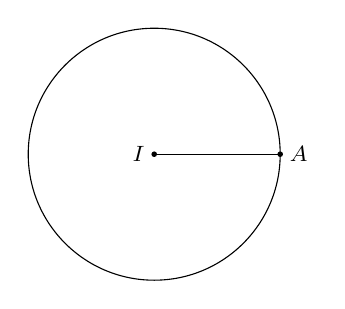
\begin{tikzpicture}[scale = 0.8, font=\footnotesize, line join=round, line cap=round, >=stealth]
				\path
				(0,0) coordinate (I)
				(2,0) coordinate (A)
				;
				\draw (I) circle (2cm);
				\draw[fill = black] (I) circle (1pt) node[left]{$I$};
				\draw[fill = black] (A) circle (1pt) node[right]{$A$};
				\draw (I)--(A);
			\end{tikzpicture}
		}
	}
\end{bt}
	\begin{bt}%[0H3K1-2]%[Yến TrầnBG10]
		Trong mặt phẳng tọa độ $Oxy$, cho tam giác $ABC$ biết $A(3; -5)$, $B(1; 3)$, $C(-2; -1)$.
		\begin{enumerate}
			\item Viết phương trình hai cạnh $AB$ và $AC$ của tam giác.
			\item Viết phương trình tổng quát của đường cao $CH$.
		\end{enumerate}
		\loigiai{
			\begin{enumerate}
				\item Ta có $\overrightarrow{AB}=(-2; 8)$ là một véc-tơ chỉ phương của đường thẳng $AB$. Suy ra $\overrightarrow{n}_{AB}=(4;1)$ là một véc-tơ pháp tuyến của $AB$. \\
				Ta lại có, đường thẳng $AB$ đi qua điểm $B(1;3)$ nên PTĐT $AB$ là $$4(x-1)+(y-3)=0\Leftrightarrow 4x+y-7=0.$$
				Ta có $\overrightarrow{AC}=(-5; 4)$ là một véc-tơ chỉ phương của đường thẳng $AC$. Suy ra $\overrightarrow{n}_{AC}=(4;5)$ là một véc-tơ pháp tuyến của $AC$. \\
				Ta lại có, đường thẳng $AC$ đi qua điểm $A(3;-5)$ nên PTĐT $AC$ là $$ 4(x-3)+5(y-(-5))=0\Leftrightarrow 4x+5y+13=0.$$
				\item Đường cao $CH\perp AB$ nên nhận véc-tơ $\overrightarrow{AB}=(-2; 8)$ là véc-tơ pháp tuyến. Suy ra $\overrightarrow{u}_{CH}=(1;-4)$ cũng là một véc-tơ pháp tuyến của $CH$. Ta lại có, đường cao $CH$ đi qua điểm $C(-2;-1)$ nên phương trình đường cao $CH$ là
				$(x-(-2))-4(y-(-1))=0\Leftrightarrow x-4y-2=0$.
			\end{enumerate}
		}
	\end{bt}
	\begin{bt}%[0H3G1-6]%[Yến TrầnBG10]
		Cho tam giác nhọn $ABC$ nội tiếp đường tròn tâm $I$. Điểm $M(2;-1)$ là trung điểm $BC$ và điểm $E\left( \dfrac{31}{13}; -\dfrac{1}{13}\right)$ là hình chiếu vuông góc của $B$ trên đường thẳng $AI$. Biết đường thẳng $AC$ có phương trình $3x+2y-13=0$, tìm tọa độ đỉnh $A$.
		
		\loigiai{
			\begin{center}
				\begin{tikzpicture}[scale=1.2, font=\footnotesize, line join=round, line cap=round, >=stealth]
					\tkzInit[xmin=-1,xmax=5,ymin=-2,ymax=4]
					\tkzClip
					\tkzDefPoints{0/0/B, 0.5/3/A, 4/0/C}
					\tkzCircumCenter(A,B,C)\tkzGetPoint{I}
					\tkzDrawCircle[radius](I,A)
					\tkzDefMidPoint(B,C)\tkzGetPoint{M}
					\tkzDefPointBy[projection= onto A--I](B)\tkzGetPoint{E}
					\tkzInterLL(E,M)(A,C)\tkzGetPoint{H}
					\tkzDrawSegments(A,B B,C C,A A,I B,E M,H B,H I,M B,I)
					\tkzDrawPoints[fill=black](I,A,B,M,C,E,H)
					\tkzLabelPoints[right](C,E,I)
					\tkzLabelPoints[above](A,H)
					\tkzLabelPoints[below](M)
					\tkzLabelPoints[left](B) 
					\tkzMarkRightAngles[size=.15](B,E,I B,M,I)
				\end{tikzpicture}
			\end{center}
			\vspace{-1cm}
			\begin{itemize}
				\item Gọi $H$ là giao điểm của $ME$ và $AC$.
				\item $\widehat{AIB}=2\widehat{ACB}$ (góc ở tâm và góc nội tiếp cùng chắn cung $AB$). \quad $(1)$
				\item $\widehat{BEI}=\widehat{BMI}=90^\circ$ nên $BMIE$ nội tiếp đường tròn đường kính $BI$, suy ra $\widehat{BIE}=\widehat{BME}$. \quad $(2)$
				\item Từ $(1)$ và $(2)$ suy ra $\widehat{BME}=2\widehat{ACB}$.
				\item Mặt khác, $\widehat{BME}$ là góc ngoài của tam giác $\widehat{HMC}$ nên $\widehat{BME}=\widehat{MHC}+\widehat{MCH}$.
				\item Suy ra $\widehat{MHC}+\widehat{MCH}=2\widehat{ACB} \Leftrightarrow \widehat{MHC}=\widehat{MCH}$. \\
				Suy ra $\triangle MHC$ cân tại $M\Rightarrow MH=MC$.
				\item Tam giác $BCH$ có $M$ là trung điểm $BC$ và $HM=MC=MB$ nên tam giác $BCH$ vuông tại $H\Rightarrow BH \perp AC$.
				\item $\overrightarrow{EM}=\left(-\dfrac{5}{13};-\dfrac{12}{13}\right) = \dfrac{-1}{13} (5;12)\Rightarrow EM$ có một véc-tơ chỉ phương $\overrightarrow{u}=(5;12)$.\\
				$\Rightarrow EM$ có một véc-tơ pháp tuyến $\overrightarrow{n}=(12;-5)$. Phương trình $EM$ là \[ 12(x-2)-5(y+1)=0 \Leftrightarrow 12x-5y-29=0.\]
				\item Tọa độ của $H$ là nghiệm của hệ phương trình \[\heva{& 3x+2y-13=0 \\ & 12x-5y-29=0} \Leftrightarrow \heva{& x=\dfrac{41}{13} \\ & y = \dfrac{23}{13}} \Rightarrow H\left(\dfrac{41}{13};\dfrac{23}{13}\right).\]
				\item $BH\perp AC$ nên đường thẳng $BH$ có dạng $2x-3y+c=0$. Do $H\in BH$ nên
				\[ 2\cdot \dfrac{41}{13} - 3\cdot \dfrac{23}{13} + c = 0 \Leftrightarrow c=-1 \Rightarrow BH \colon 2x-3y-1=0.\]
				\item Đặt $B(x;y)$. Do $M$ là trung điểm $BC$ nên $C(4-x; -2-y)$. Ta có
				\[ \heva{& B\in BH \\ & C \in AC}\Leftrightarrow \heva{& 2x-3y-1=0 \\ & 3(4-x)+2(-2-y)-13 = 0} \Leftrightarrow \heva{& x = -1 \\ & y = -1} \Rightarrow B(-1;-1), \ C(5;-1).\]
				\item $AI \perp BE$ nên $AI$ có một véc-tơ pháp tuyến là $\overrightarrow{BE}=\left(\dfrac{44}{13}; \dfrac{12}{13}\right) = \dfrac{4}{13} (11;3)$. Suy ra $AI$ có một véc-tơ pháp tuyến khác là $\overrightarrow{n}_1=(11;3)$.\\
				Phương trình $AI$ là $11  \left( x  - \dfrac{31}{13} \right) + 3  \left( y + \dfrac{1}{13}\right) = 0 \Leftrightarrow 11x + 3y -26=0$.
				\item Do $A=AI \cap AC$ nên tọa độ của $A$ là nghiệm của hệ phương trình
				\[ \heva{& 11x + 3y - 26 = 0 \\ & 3x+2y - 13 = 0} \Leftrightarrow \heva{& x = 1 \\ & y = 5} \Rightarrow A(1;5).\]
			\end{itemize}
		}
	\end{bt}
\begin{bt}%[0H3G2-5]%[Yến Trần BG10]
	Trong mặt phẳng tọa độ $Oxy$, cho đường tròn $(C) \colon (x-2)^2 + (y-1)^2=4$ và đường thẳng $d \colon 2x+y+m=0$. Tìm các giá trị của tham số $m$ để trên đường thẳng $d$ tồn tại đúng một điểm $M$ mà qua $M$ kẻ được hai tiếp tuyến $MA$, $MB$ đến $(C)$ sao cho $\widehat{AMB}=120^\circ$, trong đó $A$ và $B$ là hai tiếp điểm.
	\loigiai{
		\immini{Đường tròn $(C)$ có tâm $I(2;1)$ và bán kính $R=2$.\\
			Gọi $\Delta$ là đường thẳng đi qua $I$ và vuông góc với đường thẳng $d$.\\
			Để trên đường thẳng $d$ tồn tại đúng một điểm $M$ mà qua $M$ kẻ được hai tiếp tuyến đến $(C)$ thì $M$ là giao điểm của $d$ với $\Delta$ và $IM>R$.\\
			Đường thẳng $d$ có một véc-tơ chỉ phương là $\vec{u}=(-1;2)$.\\
			Vì $\Delta$ vuông góc với $d$ nên $\Delta$ nhận $\vec{u}=(-1;2)$ làm véc-tơ pháp tuyến. \\
			Mà $\Delta$ đi qua điểm $I(2;1)$ nên $\Delta$ có phương trình tổng quát là $$-1(x-2) + 2(y-1)=0 \Leftrightarrow x-2y=0.$$
			Vì $\widehat{AMB}=120^\circ$ nên $\widehat{AMI}=60^\circ$. \\
			Trong tam giác vuông $AMI$, ta có $\sin 60^\circ=\dfrac{IA}{IM} \Rightarrow IM=\dfrac{4}{\sqrt{3}}>R$.
		}
		{
			\begin{tikzpicture}[>=stealth,line join=round,line cap=round,font=\footnotesize,scale=1.5]
				\coordinate[label=below:$I$](I) at (2,0);
				\fill[black] (I) circle (1pt);
				\coordinate[](N) at (0,0);
				\draw[name path=circleI] let \p1=($(N)-(I)$) in (I) circle ({veclen(\x1,\y1)});
				\coordinate[label=left:$M$](M) at (-0.3,0);
				\fill[black] (M) circle (1pt);
				% Các lệnh này dùng để vẽ tiếp tuyến của đường tròn tâm O từ điểm A ngoài đường tròn. Đặt tên hai tiếp điểm là X1, X2
				%	\draw[name path=circleO] (O) circle[radius=1cm];
				\path[name path=circleX] let \p1=($(I)-($(I)!.5!(M)$)$) in ($(I)!.5!(M)$) circle ({veclen(\x1,\y1)});
				\path[name intersections={of= circleX and circleI}] coordinate (A) at (intersection-1) coordinate (B) at (intersection-2);
				\draw (M)--(A)node[above left]{$A$}--(I)--(M)--(B)node[below left]{$B$}--(I);
				\fill[black] (A) circle (1pt) (B) circle (1pt);
				\foreach \x/\dinh/\y in {M/A/I,I/B/M} 
				\draw ($(\dinh)!3pt!(\x)$)--($(\dinh)!3pt!(\x)+(\dinh)!3pt!(\y)-(\dinh)$)--($(\dinh)!3pt!(\y)$)--(\dinh)--cycle; 
				
			\end{tikzpicture}
		}
		\noindent 	Mà $IM=\mathrm{d}(I,d)$ nên ta có $\dfrac{|2\cdot 2 + 1\cdot 1 +m|}{\sqrt{5}}=\dfrac{4}{\sqrt{3}} \Leftrightarrow m=-5\pm\dfrac{4\sqrt{15}}{3}$.
	}
\end{bt}
\Closesolutionfile{ans}
\Closesolutionfile{ansbook}
\indapan{10}{ans/ans-KT-701}